\documentclass[a4paper,12pt]{report}
\usepackage[utf8]{inputenc}
\usepackage[french]{babel}
\usepackage[top=3cm, bottom=3cm, left=2cm, right=2cm]{geometry}
\usepackage[T1]{fontenc}
\usepackage{graphicx}
\usepackage{hyperref}
\usepackage{tikz}
\usepackage{color}
\usepackage{listings}
\usepackage[final]{pdfpages} 
\definecolor{mygreen}{rgb}{0,0.6,0}
\definecolor{mygray}{rgb}{0.5,0.5,0.5}
\definecolor{mymauve}{rgb}{0.58,0,0.82}
\lstset{ %
	backgroundcolor=\color{white}, % choose the background color; you must add \usepackage{color} or \usepackage{xcolor}
	basicstyle=\footnotesize, % the size of the fonts that are used for the code
	breakatwhitespace=false, % sets if automatic breaks should only happen at whitespace
	breaklines=true, % sets automatic line breaking
	captionpos=b, % sets the caption-position to bottom
	commentstyle=\color{mygreen}, % comment style
	deletekeywords={...}, % if you want to delete keywords from the given language
	escapeinside={\%*}{*)}, % if you want to add LaTeX within your code
	extendedchars=true, % lets you use non-ASCII characters; for 8-bits encodings only, does not work with UTF-8
	frame=single, % adds a frame around the code
	keepspaces=true, % keeps spaces in text, useful for keeping indentation of code (possibly needs columns=flexible)
	keywordstyle=\color{blue}, % keyword style
	language=C++, % the language of the code
	morekeywords={*,...}, % if you want to add more keywords to the set
	numbers=left, % where to put the line-numbers; possible values are (none, left, right)
	numbersep=5pt, % how far the line-numbers are from the code
	numberstyle=\tiny\color{mygray}, % the style that is used for the line-numbers
	rulecolor=\color{black}, % if not set, the frame-color may be changed on line-breaks within not-black text (e.g. comments (green here))
	showspaces=false, % show spaces everywhere adding particular underscores; it overrides 'showstringspaces'
	showstringspaces=false, % underline spaces within strings only
	showtabs=false, % show tabs within strings adding particular underscores
	stepnumber=2, % the step between two line-numbers. If it's 1, each line will be numbered
	stringstyle=\color{mymauve}, % string literal style
	tabsize=2, % sets default tabsize to 2 spaces
	title=\lstname % show the filename of files included with \lstinputlisting; also try caption instead of title
}
%%%%%%%%%%%%%%%%%%%%%%%%%%%%%%%%%%%%%%%%%%%%%%%%%%%%%%%%%%%%%%%%%%%%%%%
\begin{document}
%%%%%%%%%%%%%%%%%%%%%%%%%%%%%%%%%%%%%%%%%%%%%%%%%%%%%%%%%%%%%%%%%%%%%%%

\begin{titlepage}
    \begin{center}
        \begin{tikzpicture}[remember picture,overlay]
            \node[xshift=5.5cm, yshift=-3.6cm] at (current page.north west) {
\includegraphics[scale=0.5]{resources/logo-insa.jpg}};
            \node[xshift=15.5cm, yshift=-3.6cm] at (current page.north west) {
\includegraphics[scale=0.8]{resources/logo-asi.png}};
        \end{tikzpicture}
        \newline{} \newline{} \newline{} \newline{}
        \huge{\bsc{Informatique Répartie}} \\
        \rule{\linewidth}{1.5pt}
        \huge{\textbf{Rapport final \\ Bureau partagé}}
        \rule{\linewidth}{1.5pt} \newline{} \newline{}
    \end{center}
    \textit{Auteurs : \hfill Evaluateur :} \\ Quentin \bsc{Diaferia} \hfill Alexandre \bsc{Pauchet} 
                                            \\ Grégoire \bsc{Gutzwiller}
                                            \\ Florian \bsc{Lepetit}
                                            \\ Guillaume \bsc{Minette de Saint-Martin}
                                            \\ Elisoa \bsc{Ramarokoto}
                                            \\ Hélène \bsc{Soudry}
                                            \\
                                            \\

    \large{\underline{Cadre du projet : }} \\ \\
    \normalsize{L'objectif du projet d'informatique répartie est de permettre aux étudiants de 
        mettre en pratique les connaissances apprises en cours. Il est ainsi un parfait moyen
        de comprendre et d'appréhender les concepts importants de l'informatique répartie. Ce rapport
        a pour but de présenter l'ensemble du projet, de l'étape de spécifications au développement. En effet, 
        notre projet a consisté en le développement d'une plateforme de bureau partagé, ce qui a 
        nécessairement requis plusieurs étapes de réflexion.} \\ \\
    \begin{center}
        \textit{Date :} \\ 11 Mai 2015
    \end{center}
\end{titlepage}

%%%%%%%%%%%%%%%%%%%%%%%%%%%%%%%%%%%%%%%%%%%%%%%%%%%%%%%%%%%%%%%%%%%%%%%
\tableofcontents
%%%%%%%%%%%%%%%%%%%%%%%%%%%%%%%%%%%%%%%%%%%%%%%%%%%%%%%%%%%%%%%%%%%%%%%

\chapter*{Introduction}
\addcontentsline{toc}{chapter}{Introduction}
Notre projet d'informatique répartie portait sur un bureau virtuel partagé entre plusieurs machines. Ce rapport présente les spécifications, la conception ainsi que les choix de réalisation de ce projet.

Tout d'abord, les spécifications présentent l'ensemble des éléments devant être présents dans la livraison finale. Elles présentent également les différents cas d'utilisation de l'application.

La conception, qui découle des spécifications, décrit les éléments principaux de l'application et leurs interactions. 

Après cette étape de conception, des choix techniques sont ressorti comme étant évidents pour la réalisation du projet. Les problèmes rencontrés et les solutions trouvées à ceux-ci sont également présentées dans ce rapport.

\chapter{La phase de spécifications}
\includepdf[pages=4-11]{../conception/main.pdf}

\chapter{La phase de conception}
\includepdf[pages=4-17]{../conception/main.pdf}

\chapter{Choix techniques et phase de développement}
% Florian
% choix technologiques d'implémentation 

\chapter{Améliorations possibles}
\section{Difficultés rencontrées}

\subsection{Difficultés techniques}

\paragraph{}
L'une des difficultés que nous avons rencontrées, au niveau du développement, se situe au niveau de l'interface graphique. En effet, réaliser une interface graphique en Java, à l'aide de Swing, est une pratique que nous avons vue en cours l'année dernière, mais peu pratiquée : il a fallu nous replonger dans l'utilisation de cette librairie afin d'obtenir un rendu nous satisfaisant.

\paragraph{}
De plus, au niveau du Java également, la gestion de l'événementiel a été fastidieuse. Une fois encore, nous avons rapidement manipulé les différentes classes Java relatives aux événements il y a un an.

\paragraph{}
Au final, les problèmes majeurs de développement se sont situés au niveau de ces parties du programme et non de l'informatique répartie en elle-même, ce que nous regrettons.

\subsection{Difficultés organisationnelles}

\paragraph{}
L'un des problèmes majeurs auxquels nous avons dû faire face se situe au niveau de la communication au sein de l'équipe. En effet, le travail a du s'effectuer avec une équipe nombreuse, avec six membres, sans avoir à notre disposition une salle comme c'est le cas pour les PIC. Il nous a donc fallu utiliser des outils de gestion de projet et de communication afin de nous tenir au courant du travail des uns et des autres.

\paragraph{}
Nous avons donc utilisé les plateformes Trello, basée sur le principe du Scrumboard, et Slack, afin de nous envoyer des messages sur le projet en dehors des créneaux de cours dédié à celui-ci. Cependant, du fait de notre méconnaissance de ces outils, leur usage n'a pas été optimal.

\paragraph{}
L'absence de hiérarchie au sein de l'équipe a également posé quelques problèmes.

\section{Améliorations possibles}

\paragraph{}
Notre projet, bien que globalement fonctionnel, comporte plusieurs défauts et lacunes qui pourraient être corrigés dans le cadre d'une poursuite du projet :
\begin{itemize}
	\item La gestion des erreurs peut être grandement améliorée, via la création d'un ensemble d'exceptions et l'utilisation de fenêtres d'alertes ;
	\item Du fait du rafraîchissement du bureau tout entier lors de la modification d'un élément, le programme pourrait devenir assez lent en cas de rajout d'utilisateurs ou de widgets : il serait alors intéressant d'affiner la mise à jour du bureau en gérant indépendemment chaque widget ;
\end{itemize}

\paragraph{}
De plus, plusieurs fonctionnalités intéressantes peuvent être ajoutées :
\begin{itemize}
	\item Il est aisément possible de rajouter des widgets, selon l'imagination des développeurs ;
	\item De fonctionnalités relatives à l'interface graphique peuvent être ajoutés : redimensionnement et réduction des fenêtres, gestion de raccourcis sur le bureau, ou toute autre fonction s'inspirant des bureaux d'OS comme Ubuntu ou Windows ;
	\item 
\end{itemize}




\chapter{Répartition des tâches}
\begin{center}
	\begin{figure}
		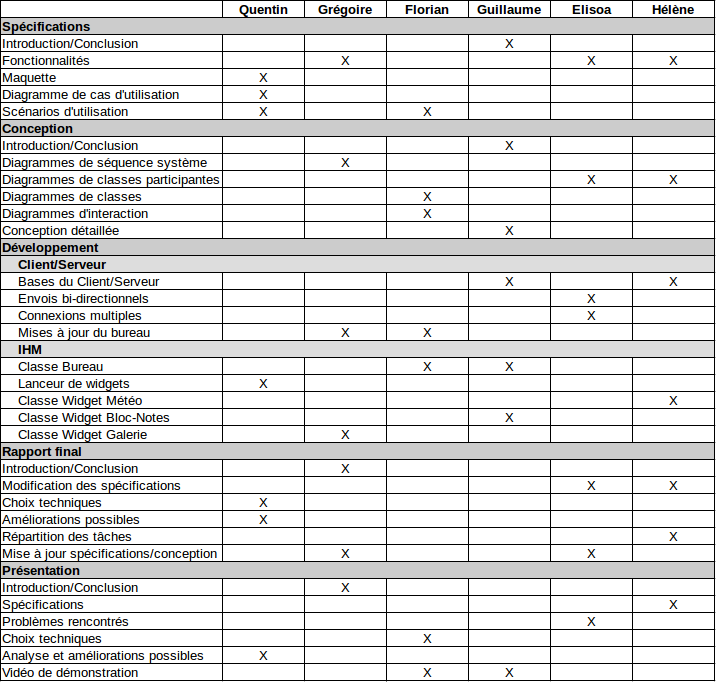
\includegraphics[scale=0.65]{resources/repartition.png}
		\caption{Répartition des tâches entre les membres du groupe}
	\end{figure}
\end{center}

\chapter*{Conclusion}
\addcontentsline{toc}{chapter}{Conclusion}
Le projet d'informatique répartie nous permet de développer un projet de A à Z. Il nous force à faire des choix technologiques en fonction des spécifications et de la conception que nous avons réalisé auparavant. De cette façon, ce projet nous a appris l'importance des étapes de conception et de spécification. 

Les premières étapes nous ont forcé à faire des choix de spécifications et de conception, ce qui est différent de la plupart des projets auxquels nous avons participé jusqu'ici.

La mise en pratique des concepts abordés lors des cours d'informatique répartie nous a permis de mieux comprendre les technologies utilisées. 

\end{document}